% Article for Revista 3i (UPDS) - same format as "Articulo Cientifico-Revista 3i.docx":
% Arial 12 pt, letter, 1 in margins, 1.5 line spacing, no indents, justified, centred bold headings,
% no page numbers, no footnotes, APA 7 references with hanging indent.
% Compile: pdflatex main.tex (run twice). No external .bib needed.
\documentclass[12pt,letterpaper]{article}
\usepackage[T1]{fontenc}
\usepackage[utf8]{inputenc}
\usepackage[spanish,es-noshorthands]{babel}
\usepackage{helvet}
\renewcommand{\familydefault}{\sfdefault}
\usepackage[margin=1in]{geometry}
\usepackage{amsmath}
\usepackage{microtype,booktabs,array,url,graphicx,xcolor}
\usepackage[hidelinks]{hyperref}
\usepackage{titlesec,setspace,caption,etoolbox,needspace}
\usepackage[round,authoryear]{natbib}
\renewcommand{\refname}{Referencias}
\setlength{\bibhang}{0.5in}          % APA hanging indent (sangr\'ia francesa)
\setlength{\bibsep}{6pt}
\pagestyle{empty}                      % the template footer is empty
\setstretch{1.43}                      % Word "1.5 lines" for Arial 12 pt
\setlength{\parindent}{0pt}
\setlength{\parskip}{6pt}
\urlstyle{same}
\Urlmuskip=0mu plus 1mu\relax
\definecolor{tm}{HTML}{001F5F}         % title colour used in the template
\titleformat{\section}{\bfseries\normalsize\centering}{}{0pt}{}
\titlespacing*{\section}{0pt}{18pt}{4pt}
\titleformat{\subsection}{\bfseries\normalsize}{}{0pt}{}
\titlespacing*{\subsection}{0pt}{18pt}{4pt}
\newcommand{\todo}[1]{\textcolor{red}{[#1]}}

% APA-style table: bold label, italic title, rules only, note below
\newenvironment{apatable}[2]{%
  \par\begin{minipage}{\linewidth}\raggedright\setstretch{1.15}
  \textbf{Tabla #1}\\[0.2em]\textit{#2}\par\vspace{0.3em}\small
}{\end{minipage}\par\vspace{6pt}}
% APA-style figure: bold label, italic title, picture, note below
\newenvironment{apafigure}[2]{%
  \par\begin{minipage}{\linewidth}\raggedright\setstretch{1.15}
  \textbf{Figura #1}\\[0.2em]\textit{#2}\par\vspace{0.4em}
}{\end{minipage}\par\vspace{6pt}}
\newcommand{\nota}[1]{\par\vspace{0.3em}{\small\textbf{\textit{Nota.}} #1}\par}

% Abstract blocks: indented 0.5 in, tighter line spacing (as in the template)
\newenvironment{absblock}{\par\begingroup\setstretch{1.09}\leftskip=0.5in\rightskip=0.1in}{\par\endgroup}
\newcommand{\absheading}[1]{\par\vspace{6pt}\noindent\textbf{#1}\par}

\begin{document}
\begin{center}
{\color{tm}\bfseries\fontsize{16}{19}\selectfont Artículo científico\par}
\vspace{10pt}
{\bfseries\fontsize{14}{17}\selectfont Clasificación del tueste del café con visión artificial y Teachable Machine\par}
\vspace{6pt}
{\itshape\setstretch{1.3} Coffee roast level classification using computer vision and Teachable Machine\par}
\vspace{4pt}
{\itshape\setstretch{1.3} Classificação do grau de torra do café com visão computacional e Teachable Machine\par}
\vspace{14pt}
{\setstretch{1.15}
\textbf{Mauri Yeison Alba Rodríguez}\\
Facultad de Ingeniería\\
Universidad Católica Boliviana\\
\href{https://orcid.org/0009-0001-3773-8549}{\textcolor{blue}{\underline{https://orcid.org/0009-0001-3773-8549}}}\\
mauri.alba@ucb.edu.bo\par}
\end{center}

\vspace{4pt}
\noindent Recibido: 17-10-2026


\absheading{Resumen}
\begin{absblock}
El objetivo de la investigación fue construir un prototipo funcional que clasifique el nivel de tueste de granos de café a partir de fotografías con Teachable Machine; el alcance de esta primera etapa se limita a capturar imágenes, entrenar el modelo y verificarlo, y deja la acción física automatizada para una etapa posterior. Se desarrolló un estudio aplicado con enfoque cuantitativo y diseño experimental, con 3.158 fotografías de siete clases (seis estados del grano y una clase de fondo), tomadas en una caja con iluminación controlada sobre dos fondos de papel; la colección se dividió por bloques de cinco fotos consecutivas en 2.208 para entrenamiento, 635 para validación y 315 para prueba, y el modelo se evaluó con las fotos separadas y según el fondo. Los resultados mostraron una exactitud de 99,1\,\% en validación (629 de 635) y de 99,4\,\% en prueba (313 de 315); los ocho errores aparecieron sobre el fondo blanco, con 97,2\,\% de aciertos frente a 100\,\% sobre el fondo anterior. En conclusión, el prototipo clasificó el tueste con alta exactitud en condiciones controladas, aunque el fondo influyó en el resultado, por lo que cada clase debe compartir el mismo fondo y la misma luz.

\textbf{Palabras clave:} café, tueste, visión artificial, clasificación, Teachable Machine
\end{absblock}

\absheading{Abstract}
\begin{absblock}
The objective of the research was to build a functional prototype that classifies the roast level of coffee beans from photographs using Teachable Machine; the scope of this first stage is limited to capturing images, training the model, and verifying it, leaving the automated physical action for a later stage. An applied study with a quantitative approach and an experimental design was conducted, using 3,158 photographs of seven classes (six bean states and one background class) taken in a box with controlled lighting on two paper backgrounds; the collection was split into blocks of five consecutive photos: 2,208 for training, 635 for validation, and 315 for testing, and the model was evaluated on the held-out photos and by background. The results showed an accuracy of 99.1\,\% in validation (629 of 635) and 99.4\,\% in testing (313 of 315); all eight errors occurred on the white background, with 97.2\,\% correct versus 100\,\% on the earlier background. In conclusion, the prototype classified roast level with high accuracy under controlled conditions, although the background influenced the result, so every class must share the same background and lighting.

\textbf{Keywords:} coffee, roasting, computer vision, classification, Teachable Machine
\end{absblock}

\absheading{Resumo}
\begin{absblock}
O objetivo da pesquisa foi construir um protótipo funcional que classifique o nível de torra de grãos de café a partir de fotografias com o Teachable Machine; o escopo desta primeira etapa limita-se a capturar imagens, treinar o modelo e verificá-lo, deixando a ação física automatizada para uma etapa posterior. Foi desenvolvido um estudo aplicado com abordagem quantitativa e delineamento experimental, com 3.158 fotografias de sete classes (seis estados do grão e uma classe de fundo), tiradas em uma caixa com iluminação controlada sobre dois fundos de papel; a coleção foi dividida em blocos de cinco fotos consecutivas: 2.208 para treinamento, 635 para validação e 315 para teste, e o modelo foi avaliado com as fotos separadas e conforme o fundo. Os resultados mostraram exatidão de 99,1\,\% na validação (629 de 635) e de 99,4\,\% no teste (313 de 315); os oito erros ocorreram sobre o fundo branco, com 97,2\,\% de acertos frente a 100\,\% sobre o fundo anterior. Em conclusão, o protótipo classificou o nível de torra com alta exatidão em condições controladas, embora o fundo tenha influenciado o resultado, de modo que cada classe deve compartilhar o mesmo fundo e a mesma luz.

\textbf{Palavras-chave:} café, torra, visão computacional, classificação, Teachable Machine
\end{absblock}


\section{Introducción}
El café es un producto de alcance mundial: la Organización Internacional del Café \citeyearpar{ico2026} estimó una producción de 177,5 millones de sacos en el año cafetero 2024 y un consumo de 175,1 millones, y el Servicio Agrícola Exterior del Departamento de Agricultura de Estados Unidos \citeyearpar{usdafas2026} proyecta para 2026/27 una producción récord de 189,7 millones de sacos y un consumo de 179,7 millones. En Bolivia, en 2025 el valor exportado fue récord, con más de 17 millones de dólares y un aumento de 13\,\% frente a 2024, aunque el volumen bajó 12\,\% y 99\,\% de lo exportado fue café sin tostar \citep{ibce2026}.

En ese contexto, el nivel de tueste define el color, el sabor y el valor del producto. La norma del Servicio de Comercialización Agrícola del Departamento de Agricultura de Estados Unidos \citeyearpar{usdaams2004} distingue cuatro tonos medidos con la escala Agtron: claro (80 a 90), medio (50 a 60), moderadamente oscuro (40 a 50) y oscuro (30 a 40), y pide que el color de los granos coincida con las lecturas del colorímetro. El tueste también pesa en el ingreso: en los Yungas, \citet{jacobi2024} registraron que el café especial verde se pagó a 2,69 dólares por libra, mientras que el tostado alcanzó entre 10,96 y 11,84 dólares por libra según el canal de venta.

Evaluar el tueste a simple vista depende de la persona: \citet{marzuki2025} señalan que la evaluación humana se ve afectada por la fatiga, la iluminación y la experiencia personal, y proponen una alternativa objetiva con imágenes. La visión artificial ya se aplicó a esta tarea: Marzuki et al. lograron 96,75\,\% de exactitud de validación con una red convolucional y cuatro niveles de tueste; \citet{anto2025} compararon cinco arquitecturas con ocho niveles Agtron sobre 2.522 imágenes tomadas con luz controlada y obtuvieron hasta 93,8\,\%; y \citet{arsyan2026} alcanzaron 96\,\% con MobileNetV2 preentrenada y cuatro niveles.

Estas redes compactas se pueden reutilizar mediante aprendizaje por transferencia \citep{howard2017,sandler2018,yosinski2014}, que es la base de herramientas sin código como Teachable Machine. Sin embargo, una exactitud alta en la prueba no siempre implica que el modelo aprendió lo que se pretendía. \citet{geirhos2020} describen los atajos como reglas de decisión que rinden bien en las pruebas habituales pero fallan en condiciones más exigentes, como las del uso real; \citet{xiao2020} muestran que el fondo de la imagen basta para clasificar con éxito razonable, y \citet{torralba2011} reportan que un clasificador de automóviles con 53,4\,\% de exactitud en su propio conjunto de datos baja a 27,5\,\% al probarlo con otros. A ello se suma la fuga de datos, que \citet{kapoor2022} identificaron en 329 artículos de 17 campos. En los estudios sobre café, \citet{arsyan2026} proponen ampliar el conjunto de imágenes con más fondos y condiciones de luz.

Este manuscrito resulta de la primera etapa de un proyecto de la asignatura Inteligencia Artificial (ISW-221) de la Universidad Católica Boliviana. El alcance de esta etapa se limita a tomar fotografías de los granos, cargarlas en Teachable Machine, entrenar el modelo y entregar un prototipo funcional; la acción física con un microcontrolador ESP32 y los requisitos que defina la asignatura corresponden a la etapa siguiente. El objetivo fue construir un prototipo que clasifique el nivel de tueste del café a partir de imágenes con Teachable Machine y comprobar si el modelo se apoya en el grano o en el fondo.

% \section{Marco teórico}
\todo{Redactar aquí: tueste y escala Agtron; visión artificial y redes convolucionales; aprendizaje por transferencia (MobileNet); sesgo de fondo y aprendizaje por atajos; métricas de evaluación.}
  % activar cuando se redacte (la plantilla de la revista no lo exige)
\section{Metodología}
Se realizó un estudio aplicado, cuantitativo y experimental, con dos tomas de fotografías. Las imágenes se tomaron en una caja cerrada por tres lados, con una cámara web USB de 1280\,\texttimes\,720 píxeles y un anillo de 16 LED controlado por un ESP32-S3 (Figura 1). La luz se ajustó a un blanco neutro-cálido, porque una luz fría daba un tinte azulado. Una foto cada 3 segundos se guardó en JPEG (calidad 92) de hasta 800 píxeles de ancho, con tres formas de colocar los granos: en grupo, dispersos e individuales.

\begin{apafigure}{1}{Montaje de captura: interior de la caja y placa ESP32-S3}
\centering
\begin{minipage}[t]{0.48\linewidth}\centering
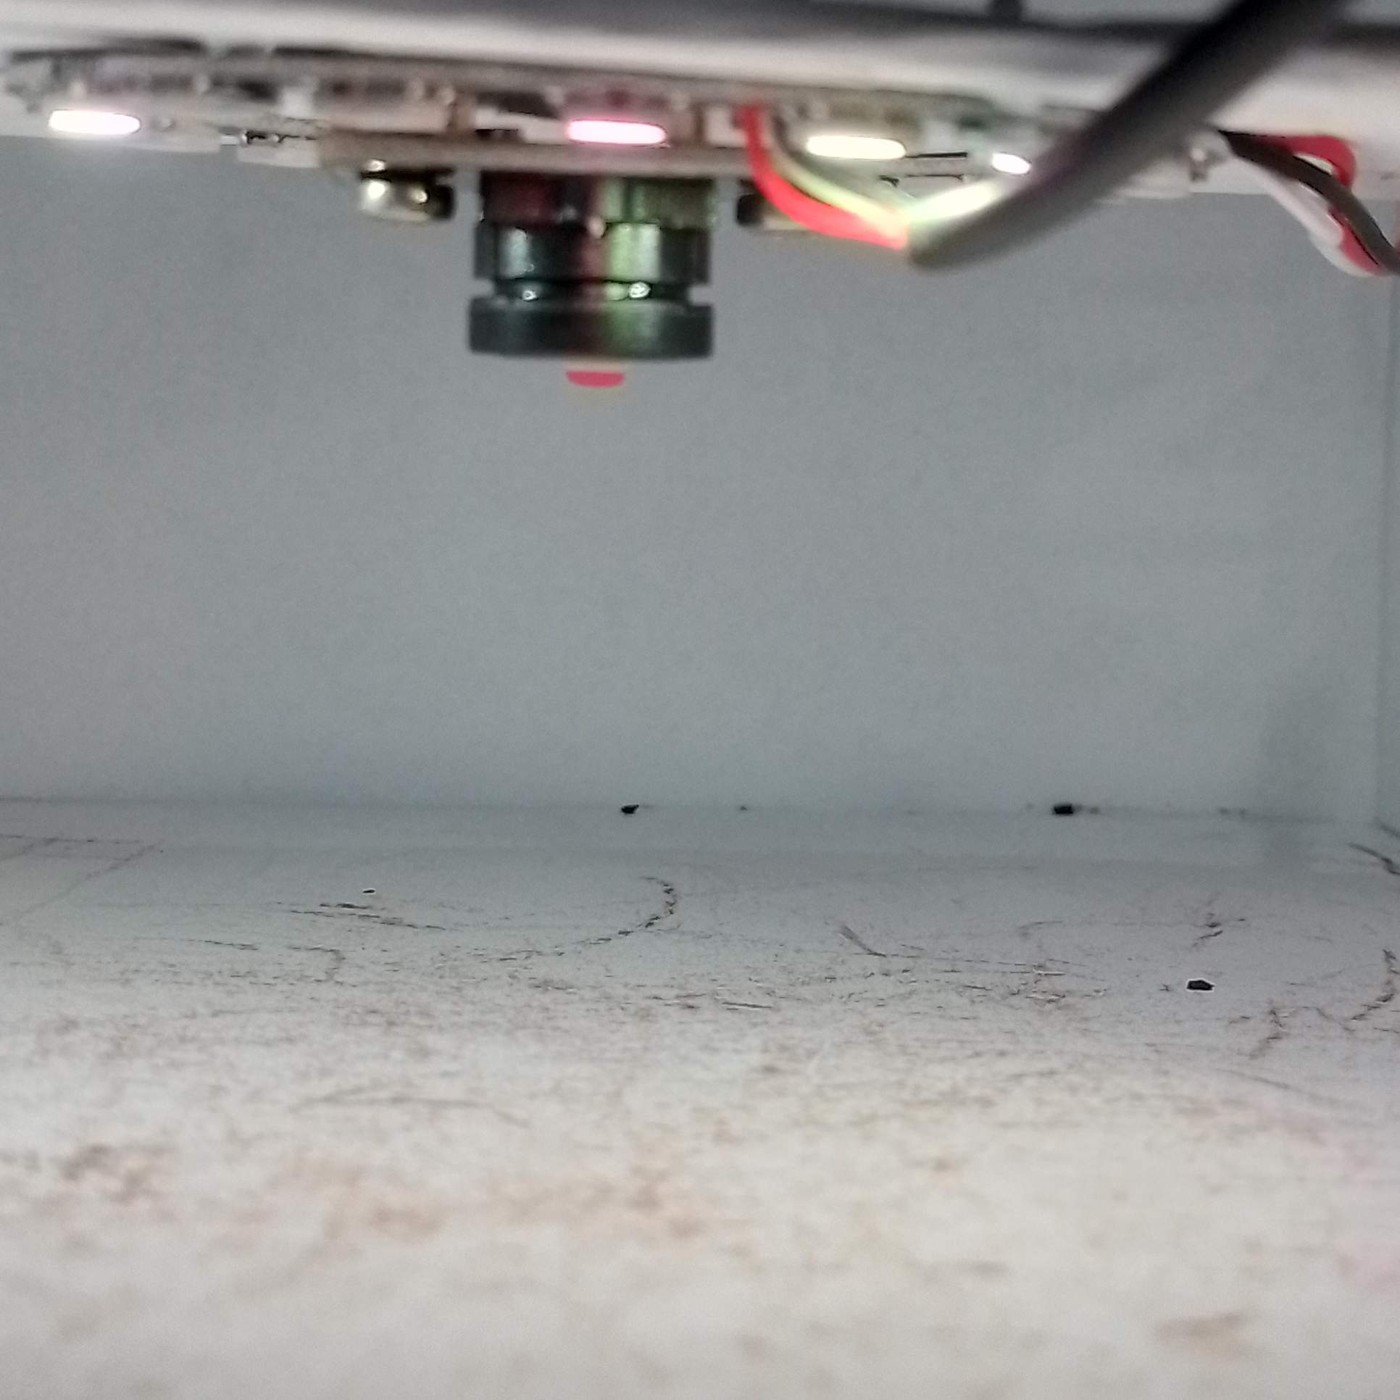
\includegraphics[width=\linewidth]{figures/fig_caja_interior.jpg}\\[2pt]{\small (a) Interior de la caja}
\end{minipage}\hfill
\begin{minipage}[t]{0.48\linewidth}\centering
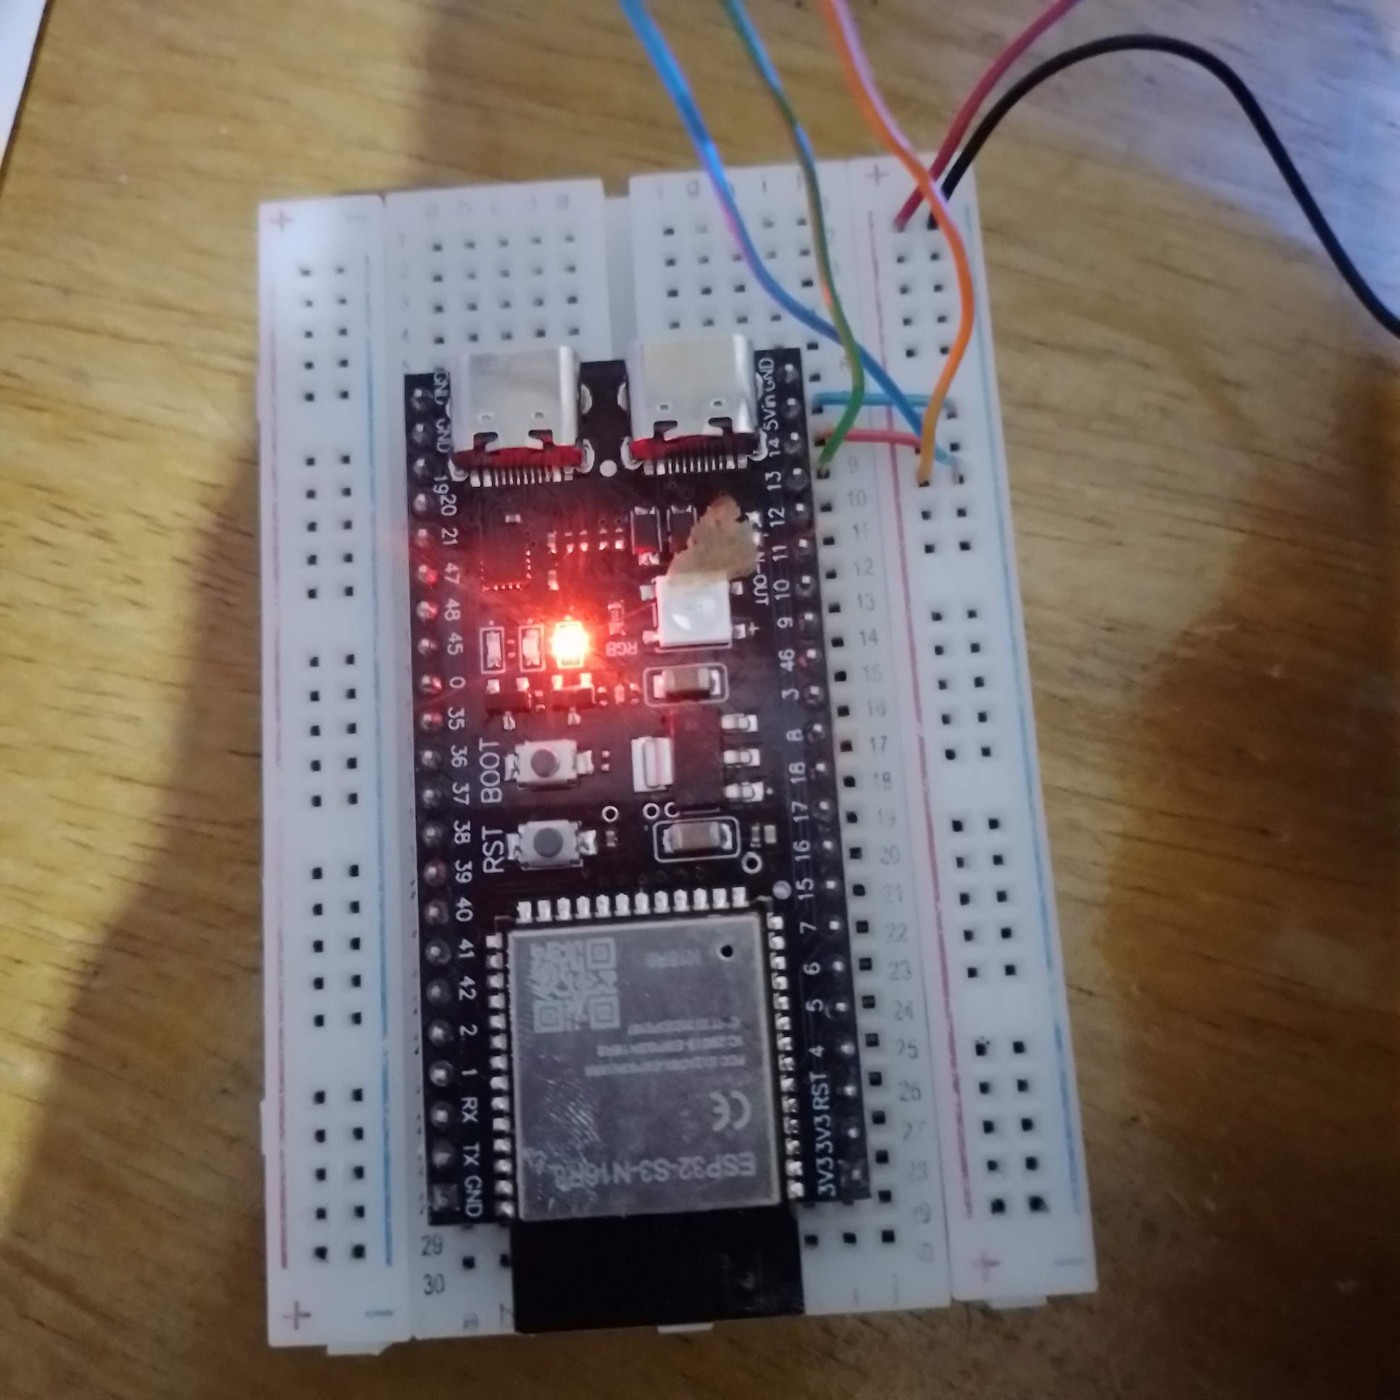
\includegraphics[width=\linewidth]{figures/fig_esp32s3.jpg}\\[2pt]{\small (b) Placa ESP32-S3}
\end{minipage}
\nota{Fotografías propias. (a) Cámara y LED en la parte superior de la caja. (b) Placa ESP32-S3 montada en una protoboard.}
\end{apafigure}

Se definieron siete clases: verde, claro, medio, medio oscuro, oscuro, quemado y fondo (papel vacío, manos y otros objetos). En la primera toma se grabaron 2.592 fotos sobre el papel inicial (verde 352, claro 370, medio 377, medio oscuro 372, oscuro 386, quemado 380 y fondo 355). Un filtrado automático con reglas propias descartó manos y guantes, fotos con pocas semillas visibles, desenfoque, mala exposición y mezcla de tuestes, y se recortó el centro de 450\,\texttimes\,450 píxeles para quitar el borde oscuro de la cámara, con lo que quedaron 2.328 fotos útiles.

En la segunda toma se volvieron a grabar todas las clases sobre una hoja blanca limpia, con la misma caja, cámara y luz, para que cada clase tuviera fotos con un mismo fondo; las fotos de la primera toma se conservaron, de modo que cada clase reúne fotos con los dos fondos. De 2.418 fotos tomadas, tras retirar capturas duplicadas en sucesión inmediata y aplicar el mismo filtrado y recorte, quedaron 830 útiles (verde 94, claro 78, medio 144, medio oscuro 123, oscuro 149, quemado 156 y fondo 86).

Las dos tomas se unieron en un conjunto de 3.158 fotos, que se dividió por bloques de cinco fotos consecutivas, ordenadas por fecha y hora de captura, para que fotos casi idénticas no quedaran a la vez en entrenamiento y prueba: 2.208 fotos de entrenamiento, 635 de validación y 315 de prueba. El orden de los bloques se mezcló con una semilla fija (42). Solo la carpeta de entrenamiento, con 2.207 fotos tras omitir un duplicado exacto, se subió a Teachable Machine; validación y prueba se guardaron para medir el modelo con fotos que nunca vio.

Se usó el modelo estándar de imágenes de Teachable Machine (224\,\texttimes\,224 píxeles en color, basado en una red tipo MobileNet) con los ajustes predeterminados de la herramienta, exportado en formato TensorFlow.js y convertido a ONNX para ejecutarlo con OpenCV sin instalar TensorFlow. Se verificó que la conversión conservó la salida del modelo original. La evaluación tuvo dos partes: la exactitud con las fotos de validación y prueba, separada según el fondo (papel inicial u hoja blanca, identificado por la fecha en el nombre de cada foto) y según la colocación de los granos (grupo, dispersos o individuales), y una prueba preliminar en vivo con la cámara del montaje, con el mismo recorte y tamaño que las fotos de entrenamiento.

Para medir el desempeño se calculó la exactitud, que es la proporción de fotografías que el modelo clasificó en la misma clase de la carpeta donde están guardadas (Ecuación 1), donde $A$ es el número de fotos acertadas y $N$ el número total de fotos evaluadas. Como la exactitud se mide con un número limitado de fotos, se calculó además su intervalo de confianza del 95 por ciento con el método de Wilson \citep{wilson1927} (Ecuación 2), donde $\hat{p}=A/N$ es la exactitud observada y $z=1{,}96$ es el valor de la distribución normal para ese nivel de confianza.

\begin{equation*}
\text{Exactitud}=\frac{A}{N}\tag*{[1]}
\end{equation*}

\begin{equation*}
\mathrm{IC}_{95}=\frac{\hat{p}+\dfrac{z^{2}}{2N}\;\pm\;z\sqrt{\dfrac{\hat{p}\,(1-\hat{p})}{N}+\dfrac{z^{2}}{4N^{2}}}}{1+\dfrac{z^{2}}{N}}\tag*{[2]}
\end{equation*}


\section{Resultados y discusión}
\textbf{Resultados}

La Tabla 1 detalla la distribución final de las 3.158 fotos; de ellas, 830 (26\,\%) son de la hoja blanca.

\begin{apatable}{1}{Imágenes por clase y por conjunto del modelo 2}
\begin{tabular}{@{}lrrrr@{}}
\toprule
Clase & Entrenamiento & Validación & Prueba & Total\\
\midrule
Verde & 300 & 83 & 40 & 423\\
Claro & 287 & 85 & 40 & 412\\
Medio & 287 & 80 & 40 & 407\\
Medio oscuro & 340 & 97 & 50 & 487\\
Oscuro & 357 & 105 & 50 & 512\\
Quemado & 331 & 95 & 50 & 476\\
Fondo & 306 & 90 & 45 & 441\\
\midrule
\textbf{Total} & \textbf{2.208} & \textbf{635} & \textbf{315} & \textbf{3.158}\\
\bottomrule
\end{tabular}
\end{apatable}

Con las fotos reservadas, el modelo 2 superó el 99\,\% de exactitud en validación y en prueba (Tabla 2). Los intervalos de confianza de los modelos 1 y 2 se solapan, por lo que no hay una diferencia estadísticamente significativa entre ellos.

\begin{apatable}{2}{Exactitud de los modelos con las fotos separadas}
\begin{tabular}{@{}llrrrc@{}}
\toprule
Modelo & Conjunto & Fotos & Aciertos & Exactitud (\%) & IC 95\,\% (\%)\\
\midrule
Modelo 1 & Validación & 470 & 468 & 99,6 & 98,5--99,9\\
Modelo 1 & Prueba & 230 & 229 & 99,6 & 97,6--99,9\\
Modelo 2 & Validación & 635 & 629 & 99,1 & 98,0--99,6\\
Modelo 2 & Prueba & 315 & 313 & 99,4 & 97,7--99,8\\
\bottomrule
\end{tabular}
\nota{Elaboración propia. Ninguna de estas fotos se usó en el entrenamiento. IC: intervalo de confianza de Wilson (Ecuación 2).}
\end{apatable}

Los ocho errores del modelo 2 fueron fotos de la hoja blanca. Seis se clasificaron como fondo (tres de quemado en grupo, dos de verde individual y una de claro en grupo) y dos de quemado en grupo se clasificaron como oscuro, con confianzas entre 0,780 y 1,000. Al separar los resultados según el fondo (Tabla 3), el modelo acertó las 663 fotos del papel inicial (100\,\%) y 279 de las 287 de la hoja blanca (97,2\,\%); los intervalos de confianza no se solapan (99,4 a 100,0\,\% frente a 94,6 a 98,6\,\%). Según la colocación de los granos, los dispersos se acertaron todos (376 de 376), los grupos en 98,8\,\% (490 de 496) y los individuales en 97,4\,\% (76 de 78), aunque en este último caso las fotos son pocas.

\begin{apatable}{3}{Exactitud del modelo 2 según el fondo y la colocación de los granos}
\begin{tabular}{@{}llrrrc@{}}
\toprule
Criterio & Grupo & Fotos & Aciertos & Exactitud (\%) & IC 95\,\% (\%)\\
\midrule
Fondo & Papel inicial & 663 & 663 & 100,0 & 99,4--100,0\\
Fondo & Hoja blanca & 287 & 279 & 97,2 & 94,6--98,6\\
\midrule
Colocación & En grupo & 496 & 490 & 98,8 & 97,4--99,4\\
Colocación & Dispersos & 376 & 376 & 100,0 & 99,0--100,0\\
Colocación & Individuales & 78 & 76 & 97,4 & 91,1--99,3\\
\bottomrule
\end{tabular}
\nota{Elaboración propia. Validación y prueba juntas (950 fotos). El fondo se identificó por la fecha en el nombre de cada foto.}
\end{apatable}

\textbf{Discusión}

Los resultados indican que el prototipo clasifica los siete grupos con alta exactitud con fotos tomadas en el montaje controlado. Los errores se concentraron en la hoja blanca (97,2\,\% frente a 100\,\% en el papel inicial), lo que es coherente con que el fondo influya en la clasificación, como describen \citet{xiao2020} para imágenes de objetos y \citet{geirhos2020} para los atajos. Esta lectura tiene límites: la hoja blanca aporta 26\,\% de las fotos, por lo que el modelo vio menos ejemplos de ese fondo, y con estos datos no se puede separar el efecto del fondo del efecto de la cantidad de fotos.

Seis de los ocho errores fueron granos clasificados como fondo, que es la clase del papel vacío. Una posible explicación es que, sobre la hoja blanca, los granos ocupan pocos píxeles y la imagen se parece a la del papel vacío; esta premisa queda como hipótesis y no se evaluó en este estudio.

A pesar de estas limitaciones vinculadas al fondo, la exactitud general es mayor que la de trabajos similares: 96,75\,\% con cuatro niveles \citep{marzuki2025}, 93,8\,\% con ocho niveles Agtron \citep{anto2025} y 96\,\% con MobileNetV2 \citep{arsyan2026}. No es una comparación directa, porque cambian las clases, los conjuntos de datos y las condiciones de captura. Además, las fotos de validación y prueba vienen del mismo montaje y de las mismas tomas que las de entrenamiento, aunque se separaron por bloques para reducir la fuga de datos \citep{kapoor2022}. Por eso la cifra describe el desempeño en condiciones controladas y no garantiza el mismo resultado con otras luces, cámaras o fondos.

Una exactitud alta con fotos guardadas no asegura el mismo resultado en uso real \citep{geirhos2020}. Además, los granos individuales están poco representados en el entrenamiento (243 fotos, 11\,\% del total de entrenamiento), y su exactitud (97,4\,\%) se midió con solo 78 fotos.


\section{Conclusiones}
Se cumplió el objetivo de la primera etapa: un modelo entrenado con Teachable Machine, basado en una red tipo MobileNet mediante aprendizaje por transferencia, clasificó los siete grupos con una exactitud de 99,1\,\% en validación (629 de 635) y de 99,4\,\% en prueba (313 de 315), lo que permite entregar un prototipo funcional. Estos valores corresponden a las condiciones controladas del montaje: los ocho errores aparecieron sobre la hoja blanca (97,2\,\% de aciertos frente a 100\,\% sobre el papel inicial), por lo que el resultado no se extiende a otras luces, cámaras o fondos.

En consecuencia, para el dispositivo final el fondo y la luz deben estandarizarse y ser los mismos para todas las clases, y el modelo debe medirse con fotos separadas por bloques. La acción física con el microcontrolador ESP32 corresponde a la etapa siguiente del proyecto.


\begin{thebibliography}{99}
\bibitem[Servicio de Comercializaci\'on Agr\'icola(2004)]{usdaams2004} Agricultural Marketing Service. (2004). \textit{Commercial item description: Coffee (A-A-20213B)}. U.S. Department of Agriculture. \url{https://www.ams.usda.gov/sites/default/files/media/CID\%20Coffee.pdf}
\bibitem[Anto et al.(2025)]{anto2025} Anto, Wibowo, Munandar, \& Salim. (2025). \textit{Comparative performance analysis of CNN architectures on coffee-bean roast classification}. TELKOMNIKA. \url{https://telkomnika.uad.ac.id/index.php/TELKOMNIKA/article/download/27090/12156}
\bibitem[Arsyan et al.(2026)]{arsyan2026} Arsyan, Kurniawardhani, \& Paputungan. (2026). \textit{Classification of roasting maturity levels of coffee beans using CNN method based on MobileNetV2}. Journal of Research in Social Science and Economics Management. \url{https://jrssem.publikasiindonesia.id/index.php/jrssem/article/download/1269/1824}
\bibitem[Servicio Agr\'icola Exterior(2026)]{usdafas2026} Foreign Agricultural Service. (2026). \textit{Coffee: World markets and trade, July 2026}. U.S. Department of Agriculture. \url{https://apps.fas.usda.gov/psdonline/circulars/2026/07/coffee.pdf}
\bibitem[Geirhos et al.(2020)]{geirhos2020} Geirhos, R., Jacobsen, J.-H., Michaelis, C., Zemel, R., Brendel, W., Bethge, M., \& Wichmann, F. A. (2020). \textit{Shortcut learning in deep neural networks}. Nature Machine Intelligence. \url{https://arxiv.org/abs/2004.07780}
\bibitem[Howard et al.(2017)]{howard2017} Howard, A. G., Zhu, M., Chen, B., Kalenichenko, D., Wang, W., Weyand, T., Andreetto, M., \& Adam, H. (2017). \textit{MobileNets: Efficient convolutional neural networks for mobile vision applications}. arXiv. \url{https://arxiv.org/abs/1704.04861}
\bibitem[Instituto Boliviano de Comercio Exterior(2026)]{ibce2026} Instituto Boliviano de Comercio Exterior. (2026). \textit{Exportaci\'on de caf\'e} (Bolet\'in Cifras N.\textordmasculine{} 1.428). \url{https://www.ibce.org.bo//images/ibcecifras_documentos/Cifras_1.428_Exportacion_de_cafe_1782396236.pdf}
\bibitem[Organizaci\'on Internacional del Caf\'e(2026)]{ico2026} International Coffee Organization. (2026). \textit{Coffee market report, February 2026}. \url{https://ico.org/documents/cy2025-26/cmr-0226-e.pdf}
\bibitem[Jacobi et al.(2024)]{jacobi2024} Jacobi, J., Lara, Opitz, et al. (2024). \textit{Making specialty coffee and coffee-cherry value chains work for family farmers' livelihoods}. World Development Perspectives. \url{https://digitalcollection.zhaw.ch/bitstream/11475/29454/3/2024_Jacobi-etal_Making-specialty-coffee-and-coffee-cherry-value-chains-work.pdf}
\bibitem[Kapoor y Narayanan(2022)]{kapoor2022} Kapoor, S., \& Narayanan, A. (2022). \textit{Leakage and the reproducibility crisis in ML-based science}. arXiv. \url{https://arxiv.org/abs/2207.07048}
\bibitem[Marzuki et al.(2025)]{marzuki2025} Marzuki, Apriani, \& Qulub. (2025). \textit{Coffee roaster maturity level classification based on convolutional neural network}. \url{https://www.iieta.org/download/file/fid/156459}
\bibitem[Sandler et al.(2018)]{sandler2018} Sandler, M., Howard, A., Zhu, M., Zhmoginov, A., \& Chen, L.-C. (2018). \textit{MobileNetV2: Inverted residuals and linear bottlenecks}. arXiv. \url{https://arxiv.org/abs/1801.04381}
\bibitem[Torralba y Efros(2011)]{torralba2011} Torralba, A., \& Efros, A. A. (2011). \textit{Unbiased look at dataset bias}. IEEE Conference on Computer Vision and Pattern Recognition. \url{https://people.csail.mit.edu/torralba/publications/datasets_cvpr11.pdf}
\bibitem[Wilson(1927)]{wilson1927} Wilson, E. B. (1927). \textit{Probable inference, the law of succession, and statistical inference}. Journal of the American Statistical Association, 22(158), 209--212. \url{https://doi.org/10.1080/01621459.1927.10502953}
\bibitem[Xiao et al.(2020)]{xiao2020} Xiao, K., Engstrom, L., Ilyas, A., \& Madry, A. (2020). \textit{Noise or signal: The role of image backgrounds in object recognition}. arXiv. \url{https://arxiv.org/abs/2006.09994}
\bibitem[Yosinski et al.(2014)]{yosinski2014} Yosinski, J., Clune, J., Bengio, Y., \& Lipson, H. (2014). \textit{How transferable are features in deep neural networks?} Advances in Neural Information Processing Systems. \url{https://arxiv.org/abs/1411.1792}
\end{thebibliography}


\subsection*{Sobre el autor}
Estudiante de Ingeniería Mecatrónica de la Universidad Católica Boliviana, sede Santa Cruz, que cursó la asignatura Inteligencia Artificial (ISW-221) en la gestión 2-2026.

\subsection*{Financiamiento de la investigación}
Con recursos propios.

\subsection*{Declaración de intereses}
Declara no tener ningún conflicto de intereses, que puedan haber influido en los resultados obtenidos o las interpretaciones propuestas.

\subsection*{Declaración de consentimiento informado}
El estudio se realizó respetando el Código de ética y buenas prácticas editoriales de publicación.

\subsection*{Derechos de uso}
Copyright\textcopyright{} 2026 por Mauri Yeison Alba Rodríguez. Este texto está protegido por la Licencia Creative Commons Atribución 4.0 Internacional.

Usted es libre para compartir, copiar y redistribuir el material en cualquier medio o formato y adaptar el documento, remezclar, transformar y crear a partir del material para cualquier propósito, incluso comercialmente, siempre que cumpla la condición de atribución: usted debe reconocer el crédito de una obra de manera adecuada, proporcionar un enlace a la licencia, e indicar si se han realizado cambios. Puede hacerlo en cualquier forma razonable, pero no de forma tal que sugiera que tiene el apoyo del licenciante o lo recibe por el uso que hace.

\end{document}
